% Left: birthday collision probability (exact) and the bound 1-exp(-n(n-1)/730). Right: coupon collector, nH_n vs simulation vs n ln n. Generated by figs_t0c08.py.
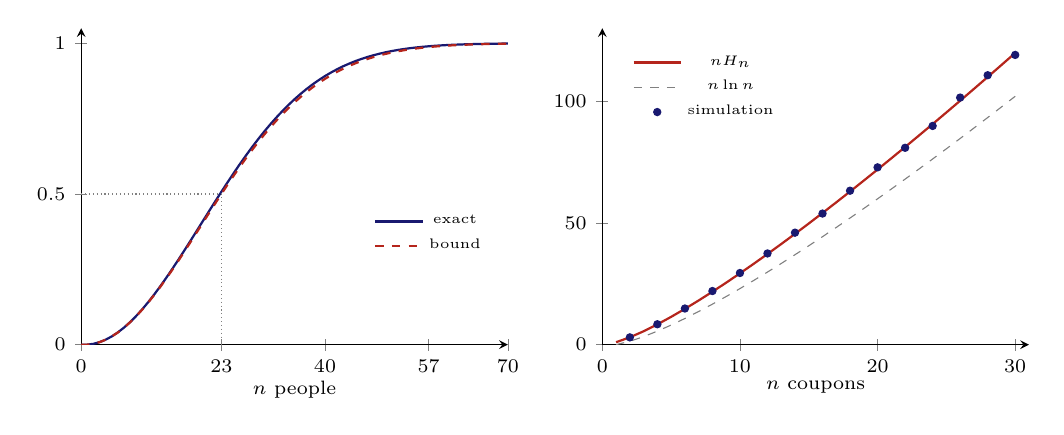
\begin{tikzpicture}
\begin{axis}[name=L,width=7cm,height=5.6cm,xmin=0,xmax=70,ymin=0,ymax=1.05,axis lines=left,xtick={0,23,40,57,70},ytick={0,0.5,1},tick label style={font=\scriptsize},xlabel={$n$ people},xlabel style={font=\scriptsize,yshift=4pt},legend style={font=\tiny,at={(0.97,0.35)},anchor=east,draw=none,fill=none}]
\addplot[MidnightBlue,thick] coordinates {(0.0000,0.00000) (1.0000,0.00000) (2.0000,0.00274) (3.0000,0.00820) (4.0000,0.01636) (5.0000,0.02714) (6.0000,0.04046) (7.0000,0.05624) (8.0000,0.07434) (9.0000,0.09462) (10.0000,0.11695) (11.0000,0.14114) (12.0000,0.16702) (13.0000,0.19441) (14.0000,0.22310) (15.0000,0.25290) (16.0000,0.28360) (17.0000,0.31501) (18.0000,0.34691) (19.0000,0.37912) (20.0000,0.41144) (21.0000,0.44369) (22.0000,0.47570) (23.0000,0.50730) (24.0000,0.53834) (25.0000,0.56870) (26.0000,0.59824) (27.0000,0.62686) (28.0000,0.65446) (29.0000,0.68097) (30.0000,0.70632) (31.0000,0.73045) (32.0000,0.75335) (33.0000,0.77497) (34.0000,0.79532) (35.0000,0.81438) (36.0000,0.83218) (37.0000,0.84873) (38.0000,0.86407) (39.0000,0.87822) (40.0000,0.89123) (41.0000,0.90315) (42.0000,0.91403) (43.0000,0.92392) (44.0000,0.93289) (45.0000,0.94098) (46.0000,0.94825) (47.0000,0.95477) (48.0000,0.96060) (49.0000,0.96578) (50.0000,0.97037) (51.0000,0.97443) (52.0000,0.97800) (53.0000,0.98114) (54.0000,0.98388) (55.0000,0.98626) (56.0000,0.98833) (57.0000,0.99012) (58.0000,0.99166) (59.0000,0.99299) (60.0000,0.99412) (61.0000,0.99509) (62.0000,0.99591) (63.0000,0.99660) (64.0000,0.99719) (65.0000,0.99768) (66.0000,0.99810) (67.0000,0.99844) (68.0000,0.99873) (69.0000,0.99896) (70.0000,0.99916)};
\addlegendentry{exact}
\addplot[BrickRed,dashed,thick] coordinates {(0.0000,0.00000) (1.0000,0.00000) (2.0000,0.00274) (3.0000,0.00819) (4.0000,0.01630) (5.0000,0.02703) (6.0000,0.04026) (7.0000,0.05591) (8.0000,0.07384) (9.0000,0.09392) (10.0000,0.11599) (11.0000,0.13988) (12.0000,0.16542) (13.0000,0.19241) (14.0000,0.22067) (15.0000,0.24999) (16.0000,0.28019) (17.0000,0.31106) (18.0000,0.34241) (19.0000,0.37406) (20.0000,0.40581) (21.0000,0.43749) (22.0000,0.46894) (23.0000,0.50000) (24.0000,0.53054) (25.0000,0.56041) (26.0000,0.58951) (27.0000,0.61774) (28.0000,0.64499) (29.0000,0.67121) (30.0000,0.69632) (31.0000,0.72028) (32.0000,0.74306) (33.0000,0.76463) (34.0000,0.78497) (35.0000,0.80410) (36.0000,0.82201) (37.0000,0.83873) (38.0000,0.85427) (39.0000,0.86868) (40.0000,0.88199) (41.0000,0.89424) (42.0000,0.90548) (43.0000,0.91575) (44.0000,0.92511) (45.0000,0.93362) (46.0000,0.94132) (47.0000,0.94827) (48.0000,0.95452) (49.0000,0.96012) (50.0000,0.96513) (51.0000,0.96960) (52.0000,0.97356) (53.0000,0.97707) (54.0000,0.98017) (55.0000,0.98290) (56.0000,0.98529) (57.0000,0.98738) (58.0000,0.98921) (59.0000,0.99079) (60.0000,0.99217) (61.0000,0.99335) (62.0000,0.99438) (63.0000,0.99526) (64.0000,0.99601) (65.0000,0.99665) (66.0000,0.99720) (67.0000,0.99766) (68.0000,0.99805) (69.0000,0.99838) (70.0000,0.99866)};
\addlegendentry{bound}
\draw[densely dotted,gray] (axis cs:0,0.5) -- (axis cs:23,0.5) -- (axis cs:23,0);
\end{axis}
\begin{axis}[at={(L.east)},anchor=west,xshift=1.2cm,width=7cm,height=5.6cm,xmin=0,xmax=31,ymin=0,ymax=130,axis lines=left,xtick={0,10,20,30},ytick={0,50,100},tick label style={font=\scriptsize},xlabel={$n$ coupons},xlabel style={font=\scriptsize,yshift=4pt},legend style={font=\tiny,at={(0.05,0.95)},anchor=north west,draw=none,fill=none}]
\addplot[BrickRed,thick] coordinates {(1.0000,1.00000) (2.0000,3.00000) (3.0000,5.50000) (4.0000,8.33333) (5.0000,11.41667) (6.0000,14.70000) (7.0000,18.15000) (8.0000,21.74286) (9.0000,25.46071) (10.0000,29.28968) (11.0000,33.21865) (12.0000,37.23853) (13.0000,41.34174) (14.0000,45.52187) (15.0000,49.77343) (16.0000,54.09166) (17.0000,58.47239) (18.0000,62.91195) (19.0000,67.40705) (20.0000,71.95479) (21.0000,76.55253) (22.0000,81.19789) (23.0000,85.88870) (24.0000,90.62300) (25.0000,95.39895) (26.0000,100.21491) (27.0000,105.06933) (28.0000,109.96079) (29.0000,114.88796) (30.0000,119.84961)};
\addlegendentry{$nH_n$}
\addplot[gray,dashed] coordinates {(1.0000,0.00000) (2.0000,1.38629) (3.0000,3.29584) (4.0000,5.54518) (5.0000,8.04719) (6.0000,10.75056) (7.0000,13.62137) (8.0000,16.63553) (9.0000,19.77502) (10.0000,23.02585) (11.0000,26.37685) (12.0000,29.81888) (13.0000,33.34434) (14.0000,36.94680) (15.0000,40.62075) (16.0000,44.36142) (17.0000,48.16463) (18.0000,52.02669) (19.0000,55.94434) (20.0000,59.91465) (21.0000,63.93497) (22.0000,68.00293) (23.0000,72.11637) (24.0000,76.27329) (25.0000,80.47190) (26.0000,84.71051) (27.0000,88.98760) (28.0000,93.30173) (29.0000,97.65158) (30.0000,102.03592)};
\addlegendentry{$n\ln n$}
\addplot[only marks,mark=*,mark size=1.3pt,MidnightBlue] coordinates {(2.0000,2.98650) (4.0000,8.37500) (6.0000,14.84150) (8.0000,22.02100) (10.0000,29.43400) (12.0000,37.46500) (14.0000,46.00350) (16.0000,53.85600) (18.0000,63.24350) (20.0000,72.84600) (22.0000,80.87100) (24.0000,89.85550) (26.0000,101.50750) (28.0000,110.69200) (30.0000,119.03250)};
\addlegendentry{simulation}
\end{axis}
\end{tikzpicture}
